\section{Template}
\begin{frame}
\frametitle{Template - Solution}
% \begin{figure}[H]
%     \centering
%     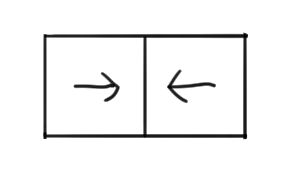
\includegraphics[scale=0.4]{./src/h.png}
% \end{figure}
\begin{block}{输入}
    a, b
\end{block}
\begin{theorem}
    $a + b = b + a$
\end{theorem}
\begin{proof}
    证明过程1 \\
    证明过程2
\end{proof}
\end{frame}

\begin{frame}[fragile]
\begin{example}
    样例1 \\
    样例2
\end{example}
\begin{block}{代码}
\begin{lstlisting}
#include <iostream>
signed main(void) {
    std::cout << a + b << std::endl;
    // comment
    return 0;
}
\end{lstlisting}
\end{block}
\end{frame}